% =====================================================================
%  CSRS -- Internship Presentation
%  Build:  ./latex/build.sh --slides      (tectonic, XeTeX)
%  Figures come from latex/figures/, shared with the work record.
% =====================================================================
\documentclass[aspectratio=169,11pt]{beamer}

\usetheme{default}
\usecolortheme{default}
\setbeamertemplate{navigation symbols}{}

% ---------- fonts -----------------------------------------------------
\usepackage{fontspec}
\usepackage[default,scale=0.96]{sourcesanspro}
\usepackage{sourcecodepro}
\usepackage{microtype}

\usepackage{graphicx}
\usepackage{booktabs}
\usepackage{tabularx}
\usepackage{array}
\usepackage{xcolor}

% ---------- palette (matches the work record) -------------------------
\definecolor{accent}{HTML}{184F95}
\definecolor{accenttint}{HTML}{E8EFF8}
\definecolor{ink}{HTML}{1A1A18}
\definecolor{soft}{HTML}{55544F}
\definecolor{rulegrey}{HTML}{D8D7D2}
\definecolor{good}{HTML}{1BAF7A}
\definecolor{warn}{HTML}{EB6834}

\setbeamercolor{normal text}{fg=ink}
\setbeamercolor{frametitle}{fg=white,bg=accent}
\setbeamercolor{itemize item}{fg=accent}
\setbeamercolor{itemize subitem}{fg=soft}
\setbeamerfont{frametitle}{size=\large,series=\bfseries}
\setbeamertemplate{itemize item}{\raisebox{0.15ex}{\tiny$\blacksquare$}}
\setbeamertemplate{itemize subitem}{\raisebox{0.15ex}{\tiny$\bullet$}}

\setbeamertemplate{frametitle}{%
  \nointerlineskip
  \begin{beamercolorbox}[wd=\paperwidth,ht=3.2ex,dp=1.4ex,leftskip=0.9em,rightskip=0.9em]{frametitle}
    \usebeamerfont{frametitle}\insertframetitle
  \end{beamercolorbox}%
  % The colour box leaves fg=white set. Paragraph text resets itself, but a
  % tabular that starts straight after the title inherits it and renders
  % white-on-white, so restore the body colour explicitly.
  \usebeamercolor[fg]{normal text}%
}

\setbeamertemplate{footline}{%
  \hbox{\begin{beamercolorbox}[wd=\paperwidth,ht=2.6ex,dp=1.1ex,leftskip=0.9em,rightskip=0.9em]{}
    \tiny\color{soft} CSRS --- Internship Presentation \hfill \insertframenumber\,/\,\inserttotalframenumber
  \end{beamercolorbox}}
}

\newcommand{\code}[1]{{\small\ttfamily #1}}
\newcommand{\lede}[1]{{\color{soft}\small #1\par\medskip}}
\newcommand{\keytake}[1]{%
  \vfill
  \noindent\colorbox{accenttint}{%
    \begin{minipage}{\dimexpr\textwidth-2\fboxsep-2\fboxrule\relax}
      \vspace{2pt}
      \small\color{accent}\textbf{#1}
      \vspace{2pt}
    \end{minipage}}\par}

\renewcommand{\arraystretch}{1.2}
\newcolumntype{L}{>{\raggedright\arraybackslash}X}
\newcolumntype{R}{>{\raggedleft\arraybackslash}X}

% =====================================================================
\begin{document}

% --- 1 ---------------------------------------------------------------
\begin{frame}[plain]
  \vspace{1.2em}
  {\color{accent}\Large\bfseries CSRS}\\[0.15em]
  {\color{soft}\large Cybersecurity Standards Retrieval System}

  \vspace{1.1em}
  {\color{rulegrey}\rule{\textwidth}{0.8pt}}
  \vspace{1.1em}

  {\large A local retrieval-augmented generation system,\\
   and what happened when it was pointed at real intrusion alerts.}

  \vspace{1.6em}
  \begin{tabular}{@{}ll@{}}
    {\color{soft}\small Intern} & \small Subhan Amir \\
    {\color{soft}\small Period} & \small 21 July -- 21 August 2026 \quad (16 working days) \\
    {\color{soft}\small Repository} & \small\ttfamily github.com/subhan-17h/CSRS \\
    {\color{soft}\small Institution} & \small\color{warn}[institution and programme] \\
    {\color{soft}\small Supervisor} & \small\color{warn}[instructor name] \\
  \end{tabular}
\end{frame}

% --- 2 ---------------------------------------------------------------
\begin{frame}{The brief}
  \lede{Build a retrieval-augmented generation system over cybersecurity standards --- and run entirely on the local machine.}
  \begin{itemize}
    \item Answer questions about cybersecurity standards \textbf{from the standards themselves}.
    \item Show where each answer came from: document, page, section.
    \item Say ``I don't know'' when the corpus does not contain the answer, rather than inventing one.
    \item Parsing, embedding, search and generation all run locally. No document content leaves the host.
  \end{itemize}
  \keytake{The offline constraint is not a detail --- it decides the model sizes, the parser, the index and the evaluation.}
\end{frame}

% --- 3 ---------------------------------------------------------------
\begin{frame}{What this presentation covers}
  \begin{columns}[T,onlytextwidth]
    \begin{column}{0.48\textwidth}
      \textbf{\color{accent}The system}\\[0.3em]
      {\small Architecture, ingestion, retrieval, generation, interfaces.}
      \vspace{1.1em}

      \textbf{\color{accent}The timeline}\\[0.3em]
      {\small 16 working days across five weeks.}
      \vspace{1.1em}

      \textbf{\color{accent}Measuring answer quality}\\[0.3em]
      {\small 50 questions, five local models, three independent metrics.}
    \end{column}
    \begin{column}{0.48\textwidth}
      \textbf{\color{accent}Applying it to real alerts}\\[0.3em]
      {\small Ranking the severity of 50 real Snort intrusion alerts --- three runs, and what each one taught.}
      \vspace{1.1em}

      \textbf{\color{accent}Honest limits}\\[0.3em]
      {\small What the system does not do, and the one result that got worse.}
    \end{column}
  \end{columns}
\end{frame}

% --- 4 ---------------------------------------------------------------
\begin{frame}{The constraint that decided everything}
  \lede{``Local'' rules out the easy version of every component.}
  \begin{itemize}
    \item \textbf{No hosted embedding API} $\rightarrow$ \code{nomic-embed-text} through Ollama, whose task prefixes are mandatory and easy to get silently wrong.
    \item \textbf{No hosted reranker} $\rightarrow$ Ollama exposes no reranking endpoint at all; FlashRank on CPU is the only option, and it ships disabled.
    \item \textbf{Small models} $\rightarrow$ 1.5B--4B parameters, so the prompt must do more work and grounding cannot be assumed.
    \item \textbf{CPU-only scoring} $\rightarrow$ BERTScore runs on CPU; the evaluation had to be resumable across hours.
  \end{itemize}
  \keytake{Every architecture choice in this project traces back to this line.}
\end{frame}

% --- 5 ---------------------------------------------------------------
\begin{frame}{System architecture}
  \begin{center}
    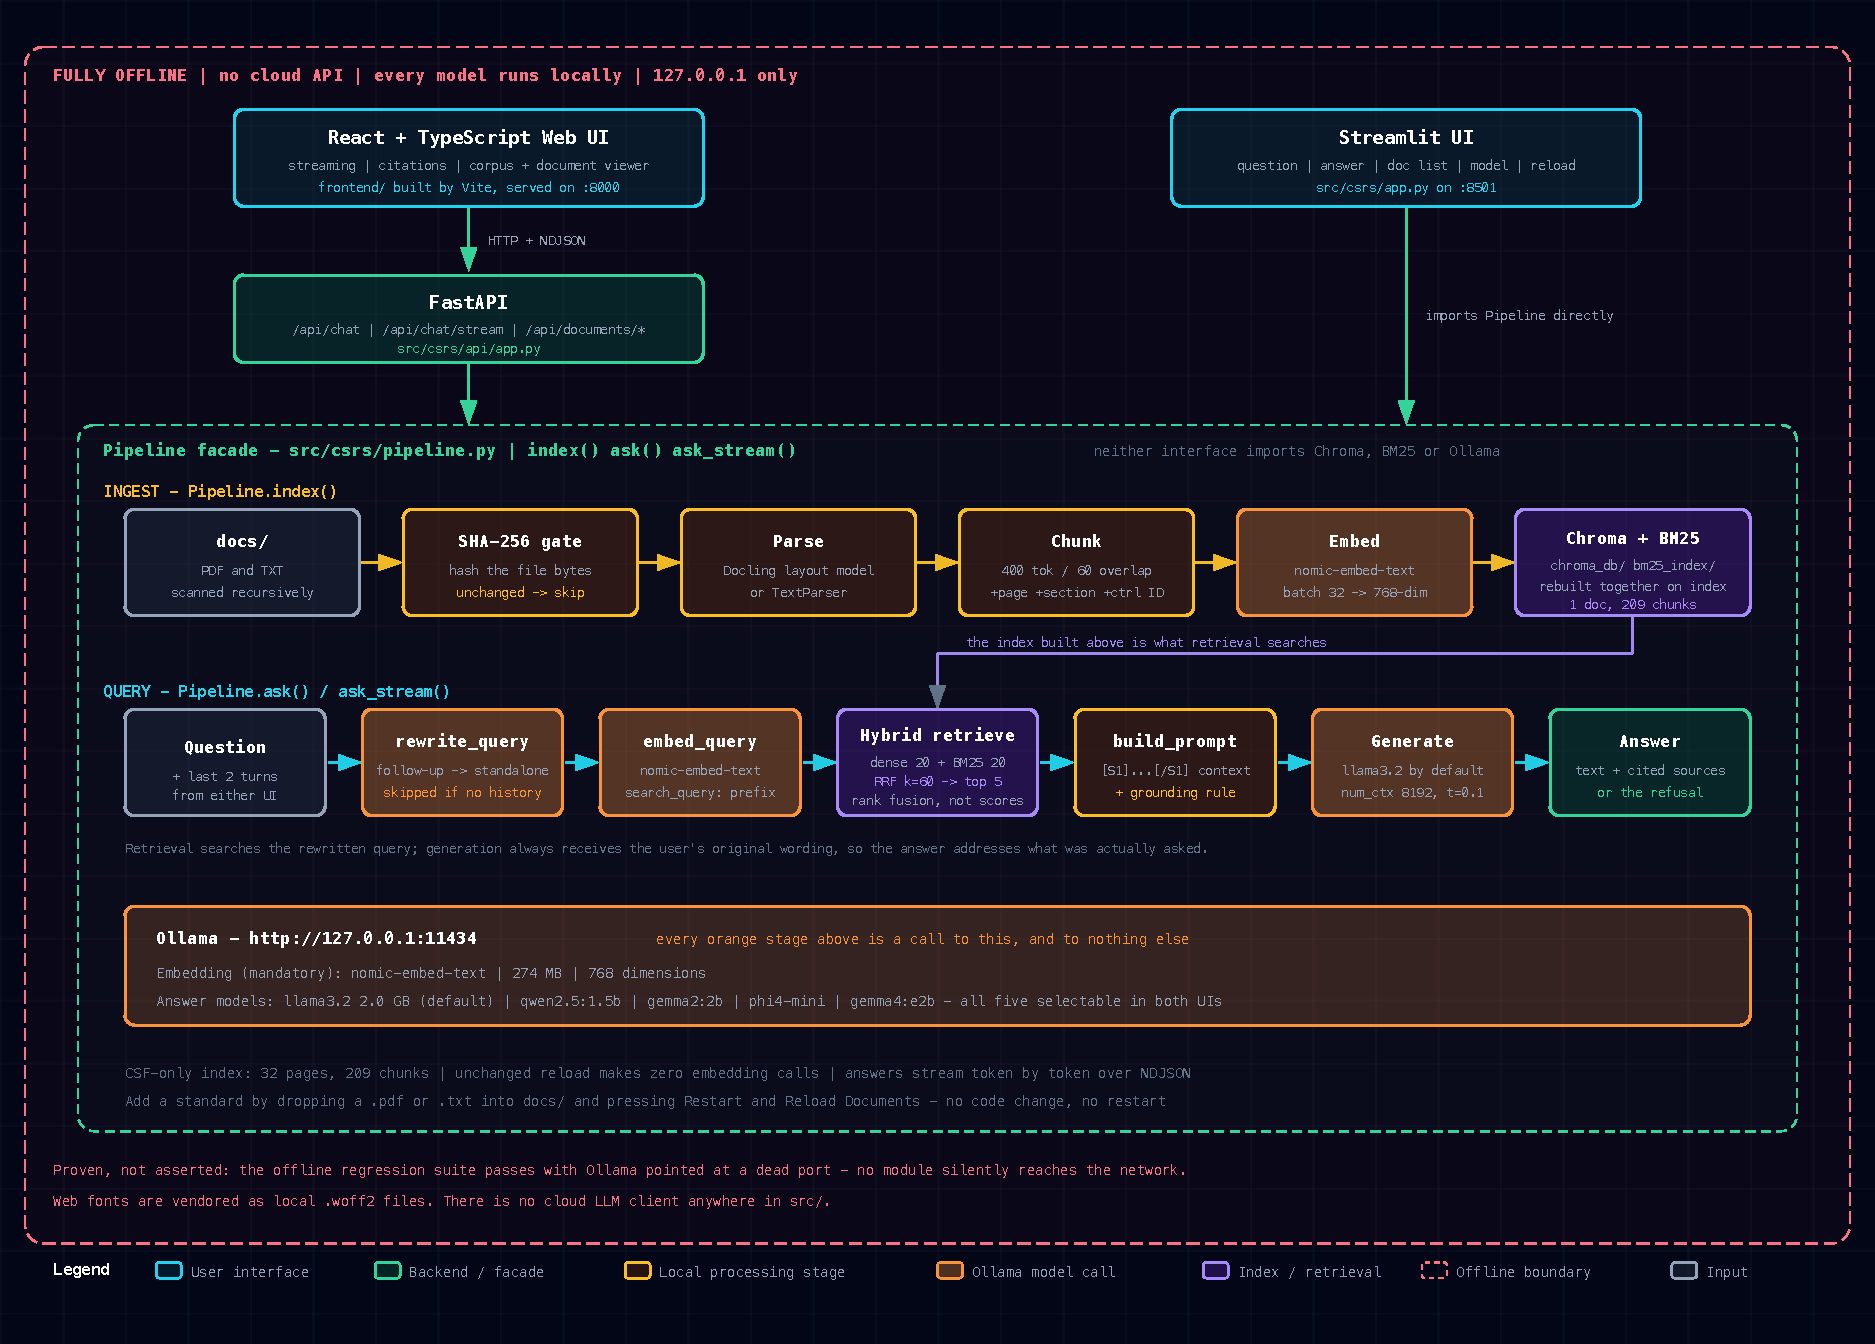
\includegraphics[width=0.92\textwidth,height=0.60\textheight,keepaspectratio]{figures/architecture.pdf}
  \end{center}
  \vspace{-0.4em}
  \lede{Everything inside the dashed boundary runs locally. The only outbound calls are the opt-in evaluation judge and the alert experiment's hosted models.}
\end{frame}

% --- 6 ---------------------------------------------------------------
\begin{frame}{Ingestion: getting a standard into the index}
  \begin{itemize}
    \item \textbf{Docling} parses PDFs with layout awareness, preserving page boundaries.
      It replaced a growing pile of hand-written cleaning heuristics --- the third time a
      new boilerplate rule was needed, the rules were the wrong answer.
    \item \textbf{Chunks carry their context}: roughly 400 tokens, each tagged with its
      heading trail and control identifier, so a retrieved passage knows where it came from.
    \item \textbf{Content-hash fingerprinting}: an unchanged corpus re-indexes in no time,
      which matters when you re-index dozens of times a day.
  \end{itemize}
  \keytake{Indexed for the experiment: 3 standards + 4,017 rule documents = 4,020 documents, 9,642 passages.}
\end{frame}

% --- 7 ---------------------------------------------------------------
\begin{frame}{Retrieval: two searches, fused}
  \begin{columns}[T,onlytextwidth]
    \begin{column}{0.46\textwidth}
      \textbf{\color{accent}Dense} --- Chroma, cosine space, our own vectors. Finds passages that \emph{mean} the same thing.
      \vspace{0.8em}

      \textbf{\color{accent}Sparse} --- a persisted BM25 index, kept in step with the corpus. Finds the passages that use the same \emph{words} --- control identifiers, rule names, CVE numbers.
    \end{column}
    \begin{column}{0.5\textwidth}
      \textbf{\color{accent}Reciprocal-rank fusion} combines the two rankings without needing their scores to be comparable.
      \vspace{0.8em}

      A measurement correction worth recording: the original target rewarded returning
      \emph{several chunks of the same control}. Re-baselining on rank-one relevance and
      Recall@5 made the improvement real rather than cosmetic --- and only then did hybrid
      retrieval become the default.
    \end{column}
  \end{columns}
  \keytake{Hybrid by default; optional CPU reranking implemented but shipped disabled.}
\end{frame}

% --- 8 ---------------------------------------------------------------
\begin{frame}{Generation: grounded, cited, and willing to refuse}
  \begin{itemize}
    \item Top passages go to a local Ollama model with a grounding instruction.
    \item The answer comes back with citations to the retrieved pages and sections.
    \item If the corpus does not support an answer, the model returns a fixed refusal string
      rather than filling the gap.
    \item Follow-up questions are rewritten against the last two turns before searching ---
      then the \emph{original} question is what the answer is generated against.
  \end{itemize}
  \keytake{A candidate pool and a generation context are different things. Only the final top evidence should spend the model's context window.}
\end{frame}

% --- 9 ---------------------------------------------------------------
\begin{frame}{Two interfaces, one pipeline}
  \begin{columns}[T,onlytextwidth]
    \begin{column}{0.49\textwidth}
      \begin{center}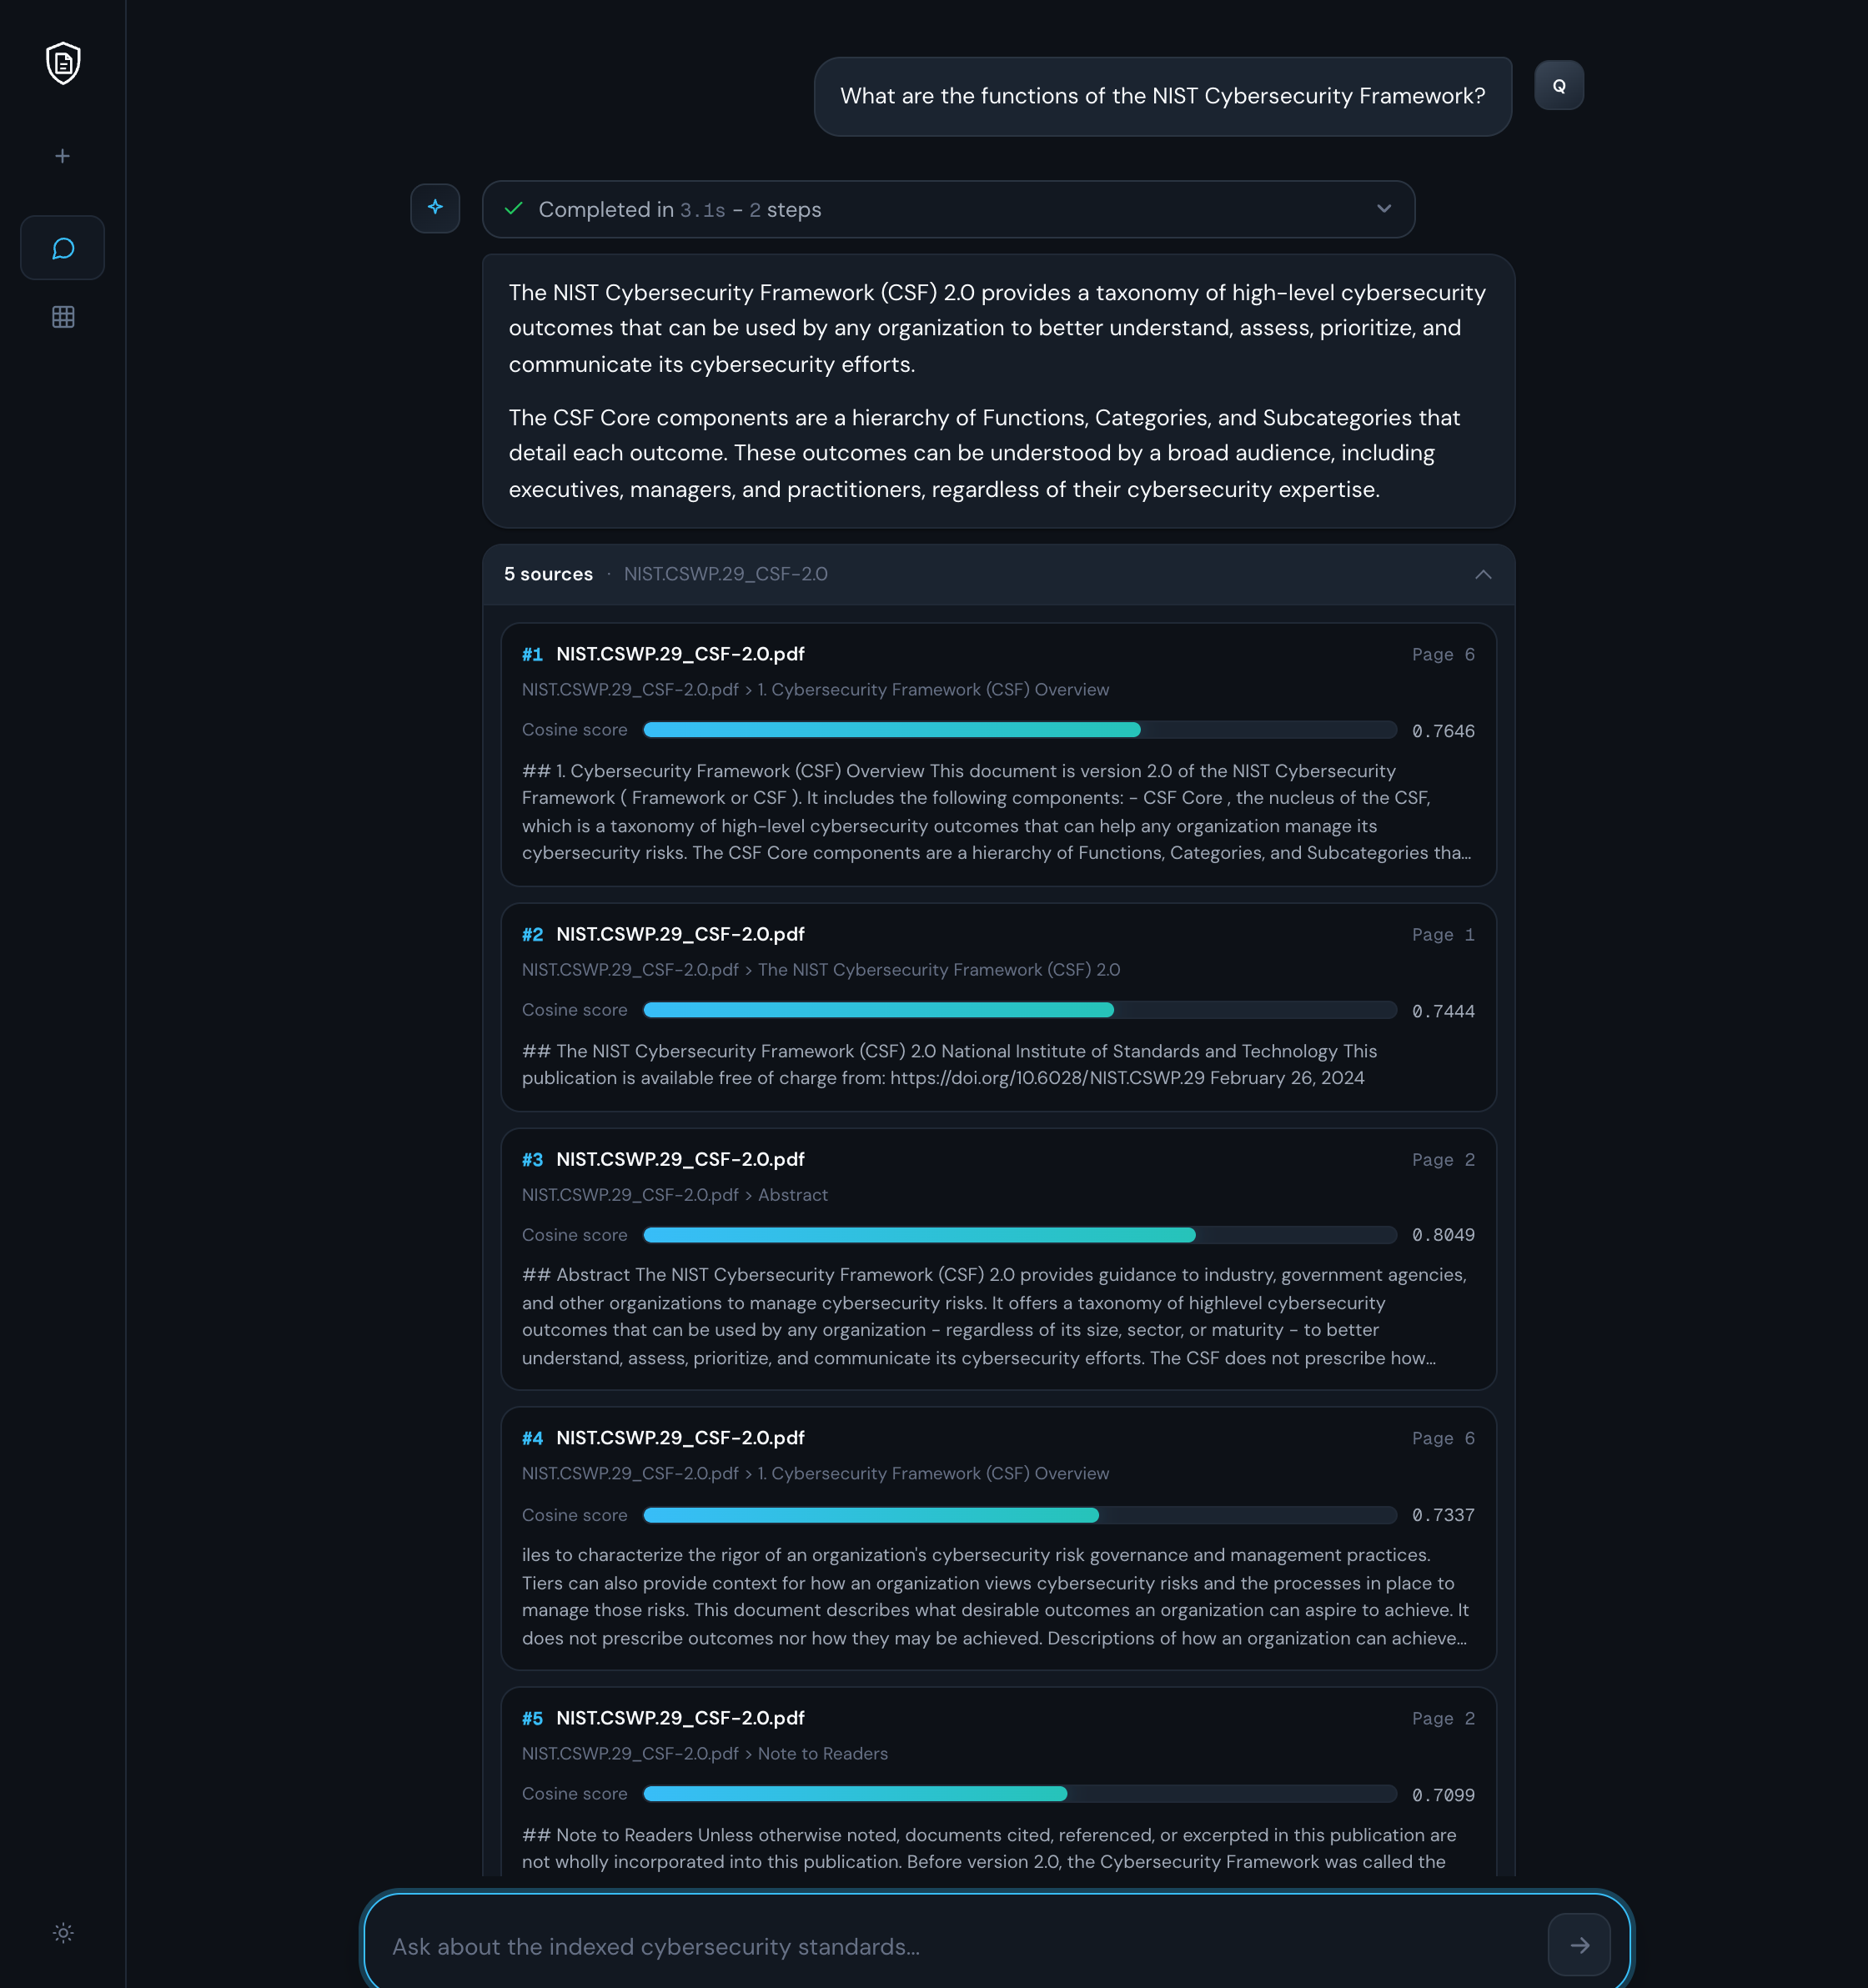
\includegraphics[width=\textwidth,height=0.58\textheight,keepaspectratio]{figures/ui_web_answer.png}\end{center}
      {\footnotesize\color{soft}React + FastAPI: streamed tokens, source cards, saved conversations, corpus browser, in-app document viewer.}
    \end{column}
    \begin{column}{0.49\textwidth}
      \begin{center}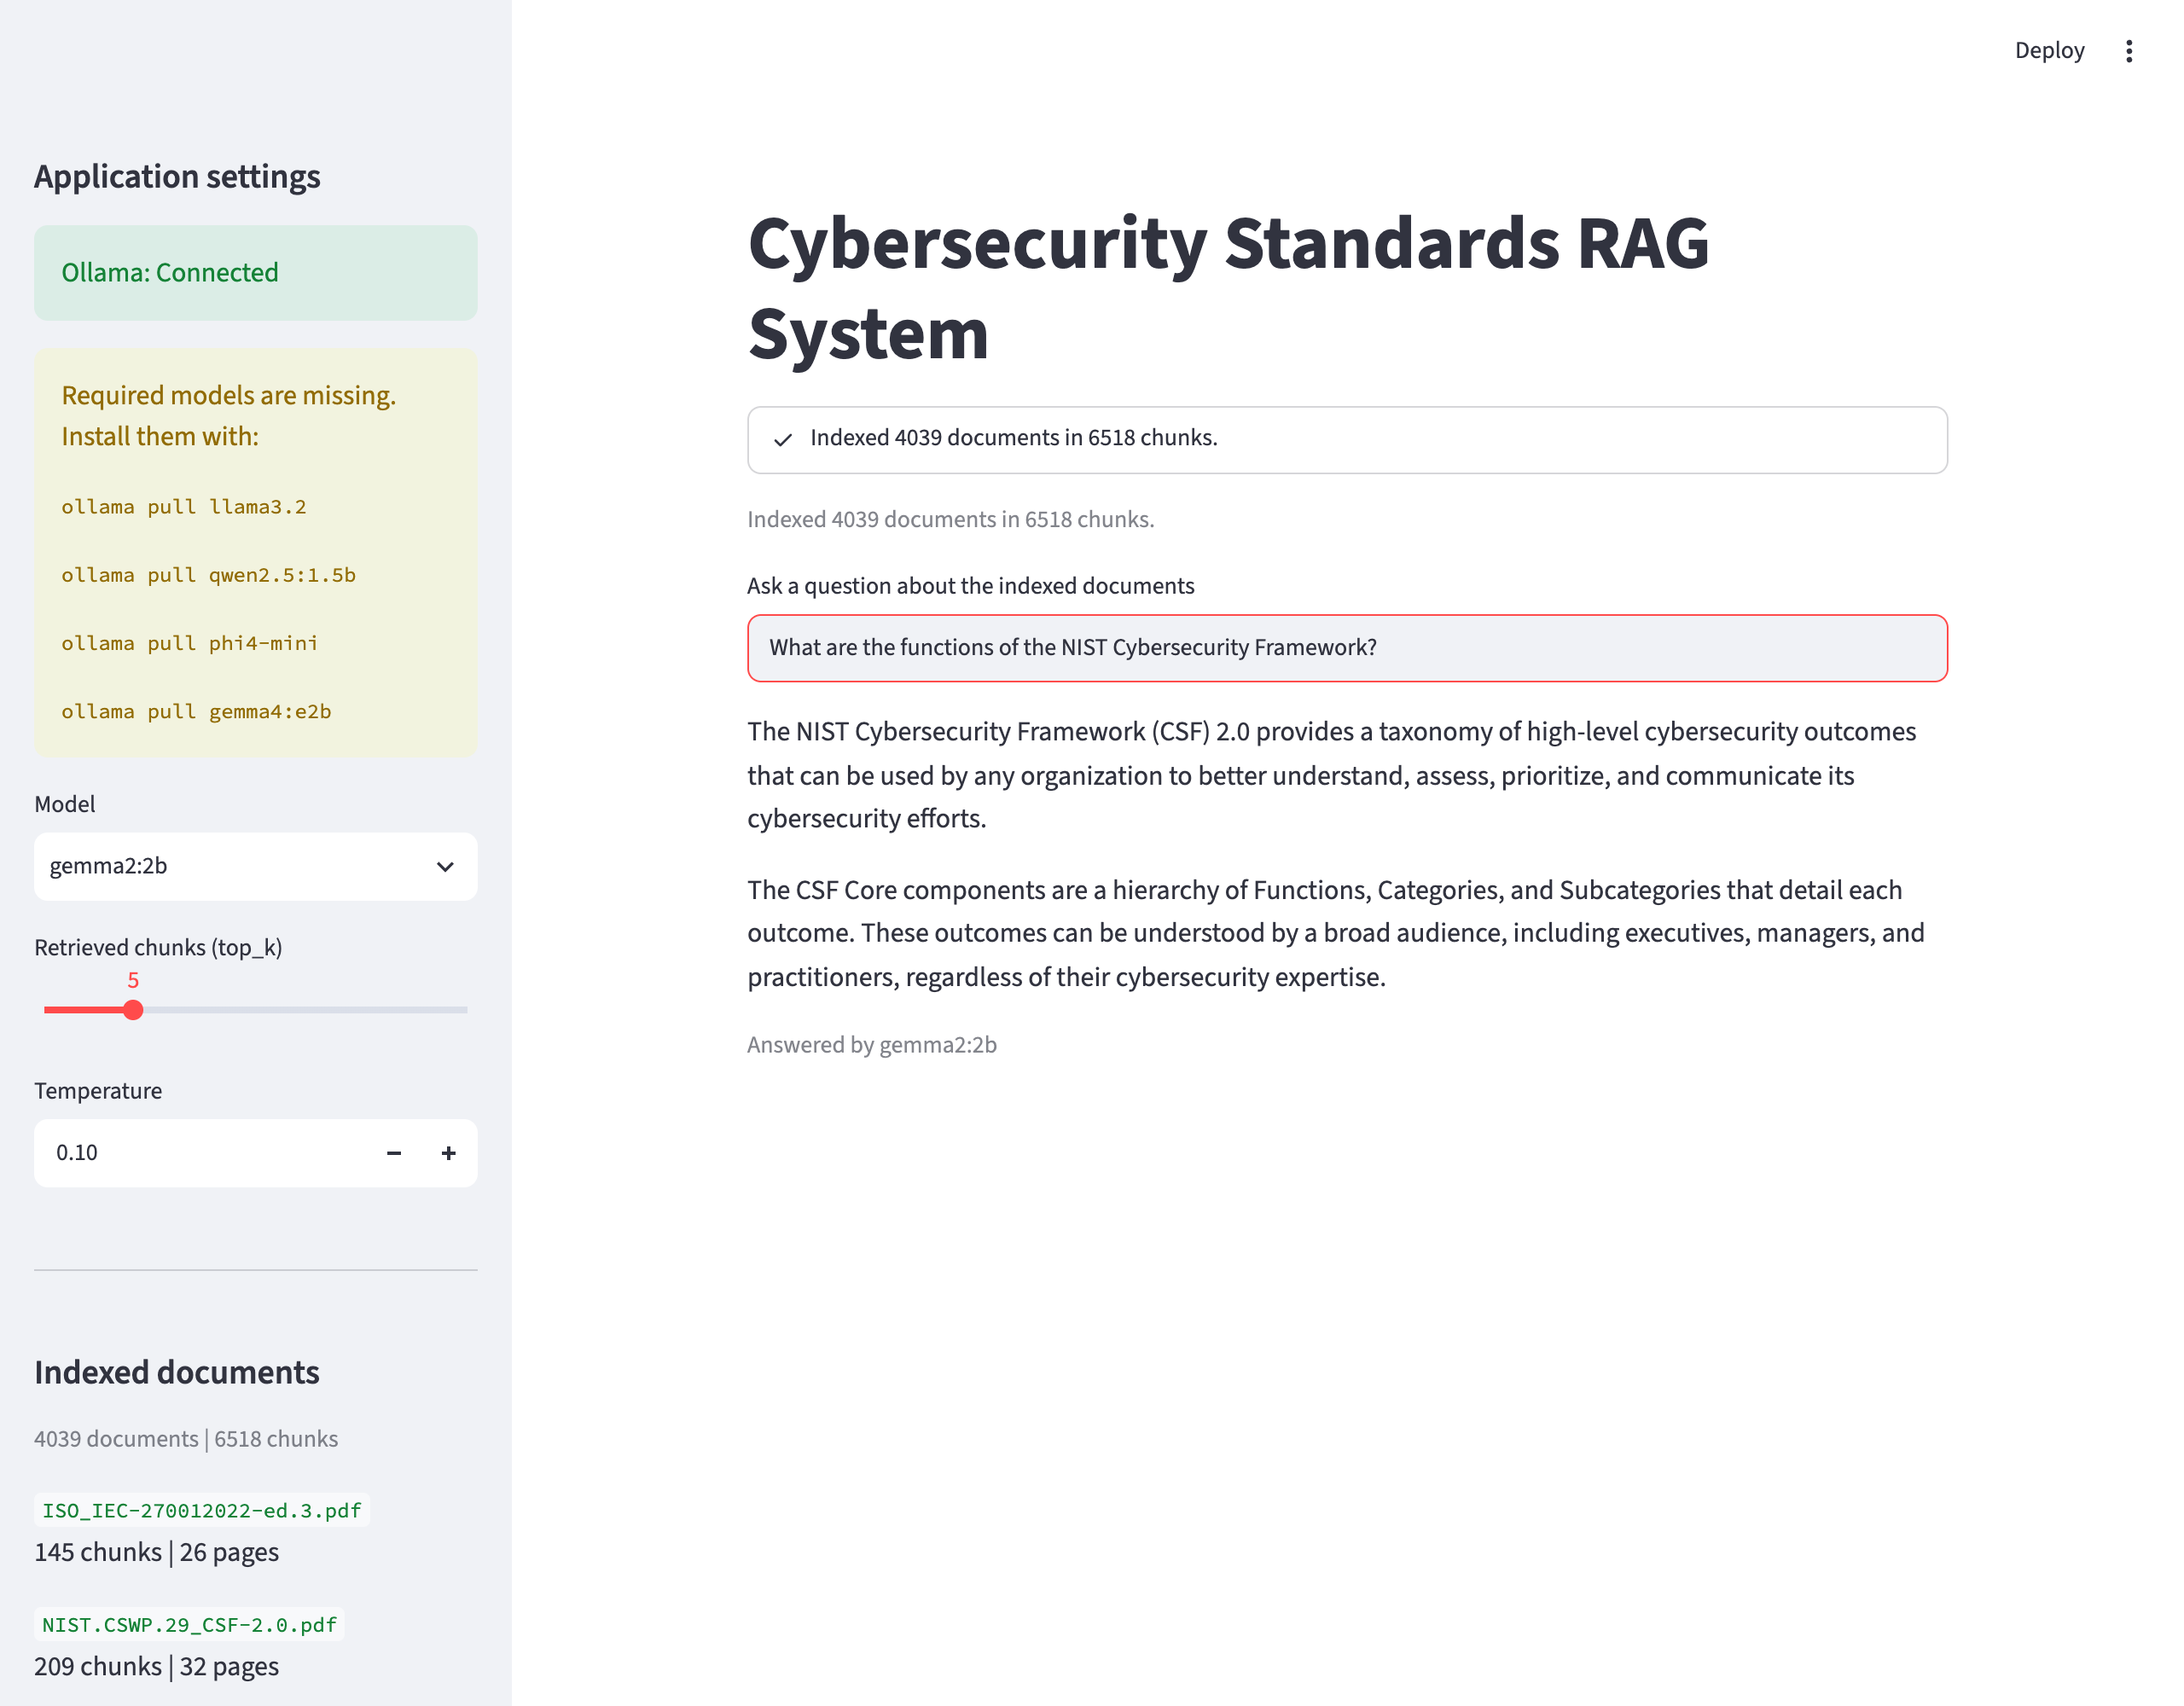
\includegraphics[width=\textwidth,height=0.58\textheight,keepaspectratio]{figures/ui_streamlit.png}\end{center}
      {\footnotesize\color{soft}Streamlit: the required local interface, same \code{Pipeline} facade, same grounded answers.}
    \end{column}
  \end{columns}
\end{frame}

% --- 10 --------------------------------------------------------------
\begin{frame}{The internship, day by day}
  \begin{center}
    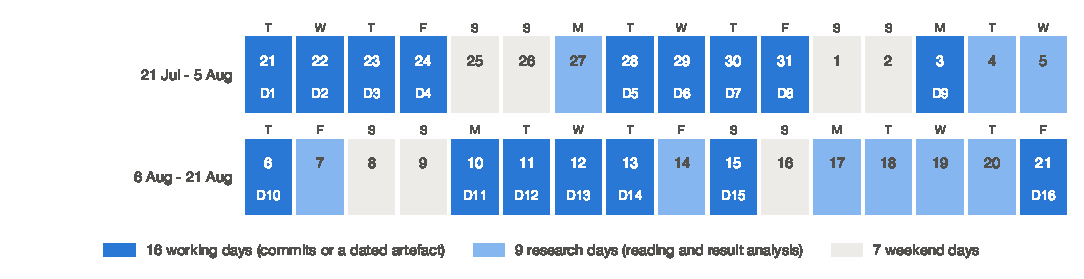
\includegraphics[width=\textwidth]{figures/calendar.pdf}
  \end{center}
  \vspace{-0.2em}
  \lede{32 calendar days. 16 working days --- on each, either commits were made or a dated
  artefact was produced. Three working days produced artefacts rather than code: the alert
  dataset, the scraping session, and the severity rubric.}
  \keytake{117 commits, each one completed task, committed only after its acceptance check passed.}
\end{frame}

% --- 11 --------------------------------------------------------------
\begin{frame}{Week 1 --- from nothing to a working system (Days 1--4)}
  % \leavevmode is required: this deck overrides the frametitle template, which
  % leaves the body in horizontal mode. A table that opens the body is then
  % swallowed and the slide renders blank. Tables inside columns are unaffected.
  \leavevmode
  {\footnotesize
  \begin{tabular}{@{}>{\raggedright\arraybackslash}p{0.085\textwidth}
                    >{\raggedright\arraybackslash}p{0.075\textwidth}
                    >{\raggedright\arraybackslash}p{0.66\textwidth}
                    >{\raggedleft\arraybackslash}p{0.085\textwidth}@{}}
    \toprule
    \textbf{Day} & \textbf{Date} & \textbf{What shipped} & \textbf{Commits} \\
    \midrule
    Day 1 & 21 Jul & Spec, roadmap and typed config; then the whole first path --- loaders, chunking, embeddings, Chroma, grounded generation, Streamlit. & 23 \\
    Day 2 & 22 Jul & Docling replaced the PDF heuristics; content-hash indexing; model warming; FastAPI and React begun. & 18 \\
    Day 3 & 23 Jul & Token streaming, settings, corpus explorer, saved conversations; both UIs verified. & 11 \\
    Day 4 & 24 Jul & Retrieval metrics, BM25, RRF, optional reranking; the metric re-baselined; hybrid became default. & 22 \\
    \bottomrule
  \end{tabular}}
  \keytake{A working RAG system with two interfaces existed at the end of week one.}
\end{frame}

% --- 12 --------------------------------------------------------------
\begin{frame}{Week 2 --- measuring it, then changing the question (Days 5--8)}
  % \leavevmode is required: this deck overrides the frametitle template, which
  % leaves the body in horizontal mode. A table that opens the body is then
  % swallowed and the slide renders blank. Tables inside columns are unaffected.
  \leavevmode
  {\footnotesize
  \begin{tabular}{@{}>{\raggedright\arraybackslash}p{0.085\textwidth}
                    >{\raggedright\arraybackslash}p{0.075\textwidth}
                    >{\raggedright\arraybackslash}p{0.775\textwidth}@{}}
    \toprule
    \textbf{Day} & \textbf{Date} & \textbf{What shipped} \\
    \midrule
    --- & 27 Jul & \emph{Research.} How retrieval quality is measured and improved. HyDE, multi-query expansion, step-back prompting and CRAG evaluated --- and declined, each for a stated reason. \\
    Day 5 & 28 Jul & EVAL-2: answer-quality evaluation replacing the retrieval-only harness. \\
    Day 6 & 29 Jul & EVAL-3: corpus cut to CSF 2.0, 50 new questions, five models, three metrics, 250 rows. \\
    Day 7 & 30 Jul & \emph{Artefact, no commit.} The 50-alert Snort dataset prepared. \\
    Day 8 & 31 Jul & \emph{Artefact, no commit.} snort.org rule documentation scraped --- 16 files. \\
    \bottomrule
  \end{tabular}}
  \keytake{Days 7 and 8 have no commits --- and they are why the second half was possible.}
\end{frame}

% --- 13 --------------------------------------------------------------
\begin{frame}{Measuring answer quality: the design}
  \lede{One document, 50 evidence-grounded questions, five local models, three metrics that do not talk to each other.}
  \begin{itemize}
    \item \textbf{Corpus reduced to NIST CSF 2.0} --- 209 chunks from 32 pages. A smaller,
      fully-known corpus makes a claim about retrieval checkable.
    \item \textbf{Cosine similarity} against a reference answer (pass $\geq$ 0.75).
    \item \textbf{BERTScore F1}, raw RoBERTa-large on CPU (pass $\geq$ 0.85).
    \item \textbf{An LLM judge} at temperature zero, opt-in and quota-safe.
  \end{itemize}
  \keytake{The three metrics are deliberately never combined into one score. They measure different things and disagree usefully.}
\end{frame}

% --- 14 --------------------------------------------------------------
\begin{frame}{Five models, three metrics, 250 rows}
  \begin{center}
    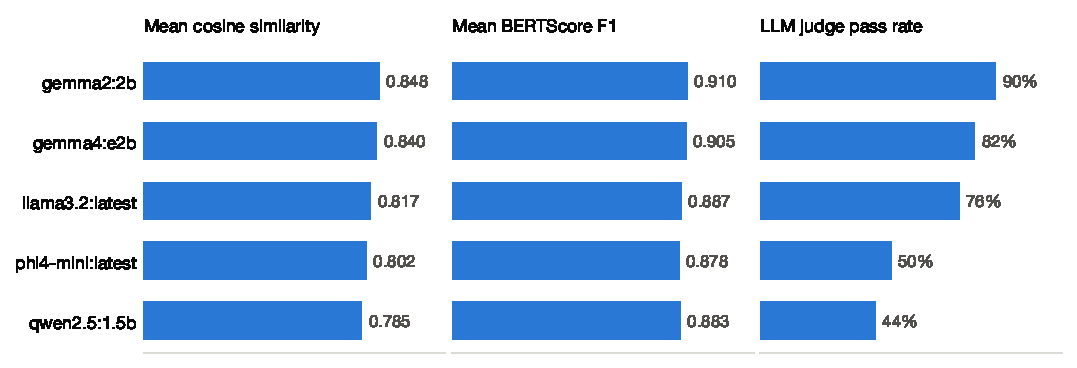
\includegraphics[width=0.86\textwidth]{figures/eval_models.pdf}
  \end{center}
  \vspace{-0.3em}
  \lede{Every cell is a real run: 50 questions per model, no technical errors, fully resumable across quota windows.}
\end{frame}

% --- 15 --------------------------------------------------------------
\begin{frame}{What the evaluation found}
  % \leavevmode is required: this deck overrides the frametitle template, which
  % leaves the body in horizontal mode. A table that opens the body is then
  % swallowed and the slide renders blank. Tables inside columns are unaffected.
  \leavevmode
  {\small
  \begin{tabularx}{\textwidth}{@{}l R R R R R@{}}
    \toprule
    \textbf{Model} & \textbf{Mean cosine} & \textbf{Cosine pass} & \textbf{Mean BERTScore} & \textbf{BS pass} & \textbf{Judge pass} \\
    \midrule
    \code{gemma2:2b}       & 0.848 & 82\% & 0.910 & 100\% & 90\% \\
    \code{gemma4:e2b}      & 0.840 & 76\% & 0.905 & 98\%  & 82\% \\
    \code{llama3.2}        & 0.817 & 74\% & 0.887 & 96\%  & 76\% \\
    \code{phi4-mini}       & 0.802 & 64\% & 0.878 & 86\%  & 50\% \\
    \code{qwen2.5:1.5b}    & 0.785 & 48\% & 0.883 & 90\%  & 44\% \\
    \bottomrule
  \end{tabularx}}
  \vspace{0.4em}
  {\small
  \begin{itemize}\setlength{\itemsep}{1pt}
    \item \code{gemma2:2b} leads on all three measures --- an unusually clean result.
    \item The judge separates models far more sharply than the embedding metrics
      (90\% vs 44\%, against 82\% vs 48\% on cosine).
  \end{itemize}}
  \keytake{A 2B model, running locally on a laptop, answers 9 in 10 questions acceptably.}
\end{frame}

% --- 16 --------------------------------------------------------------
\begin{frame}{Changing the question: from answering to triaging}
  \lede{A security analyst does not usually have a question. They have a queue.}
  \begin{itemize}
    \item \textbf{The task:} given 50 real Snort intrusion alerts, rank each one's severity
      from 1 (most severe) to 5, using retrieved standards evidence.
    \item \textbf{The catch:} the ranker sees the alert's own content --- but \emph{not} its
      rule identity and \emph{not} the rule documentation.
    \item \textbf{So:} any correct identification of the underlying rule has to come from
      what retrieval actually found. It cannot be looked up.
    \item \textbf{Ground truth:} Snort's own three-level priority, mapped onto the 1--5 scale.
  \end{itemize}
  \keytake{Same retriever, same index, entirely different question --- and a much harder one to grade.}
\end{frame}

% --- 17 --------------------------------------------------------------
\begin{frame}{First, define what ``severity'' means (Day 9)}
  \lede{Before any code: nine criteria, each with a real alert and a correct interpretation.}
  \begin{columns}[T,onlytextwidth]
    \begin{column}{0.48\textwidth}
      {\small
      \begin{enumerate}\setlength{\itemsep}{1pt}
        \item Potential impact
        \item Attack type / vector
        \item Likelihood of success
        \item Level of access gained
        \item Sensitive-data exposure
      \end{enumerate}}
    \end{column}
    \begin{column}{0.48\textwidth}
      {\small
      \begin{enumerate}\setlength{\itemsep}{1pt}\setcounter{enumi}{5}
        \item Snort priority
        \item Alert context
        \item Ease of mitigation
        \item Alert frequency
      \end{enumerate}}
    \end{column}
  \end{columns}
  \vspace{0.9em}
  {\small Two of them are traps, and the rubric says so explicitly:}
  \begin{itemize}
    \item {\small \textbf{Snort priority} is ``only a starting clue'' --- an iPhone User-Agent detection and a serious exploit can both be Priority 1.}
    \item {\small \textbf{Alert frequency} ``measures volume, not danger'' --- 304 alerts from one scanner matter less than 2 ShellShock hits.}
  \end{itemize}
\end{frame}

% --- 18 --------------------------------------------------------------
\begin{frame}{How a ranking gets graded}
  \begin{columns}[T,onlytextwidth]
    \begin{column}{0.47\textwidth}
      \textbf{\color{accent}The anchor}\\[0.3em]
      {\small Snort priority $\rightarrow$ rank:\\[0.3em]
      \quad Priority 1 $\rightarrow$ anchor 1\\
      \quad Priority 2 $\rightarrow$ anchor 3\\
      \quad Priority 3 $\rightarrow$ anchor 5}
      \vspace{0.9em}

      \textbf{\color{accent}The mismatch rule}\\[0.3em]
      {\small More than \emph{one step} from the anchor counts as a mismatch. One step is
      allowed, because the rubric explicitly wants the model to revise the priority when
      evidence justifies it.}
    \end{column}
    \begin{column}{0.49\textwidth}
      \textbf{\color{accent}The independent judge}\\[0.3em]
      {\small A \emph{different model family} scores each ranking and its justification,
      0 to 1, seeing the ground truth.}
      \vspace{0.9em}

      {\small Why it matters: in v1 the ranker judged itself and scored 0.586. Splitting
      ranker and judge across families did not make the judge kinder --- it stopped the
      rubber-stamping and exposed real errors.}
    \end{column}
  \end{columns}
  \keytake{Grading by distance from truth, not pass/fail, is what makes the later regression diagnosable.}
\end{frame}

% --- 19 --------------------------------------------------------------
\begin{frame}{v1 $\rightarrow$ v2: fixing the prompt and the judge}
  % \leavevmode is required: this deck overrides the frametitle template, which
  % leaves the body in horizontal mode. A table that opens the body is then
  % swallowed and the slide renders blank. Tables inside columns are unaffected.
  \leavevmode
  {\small
  \begin{tabular}{@{}>{\raggedright\arraybackslash}p{0.17\textwidth}
                    >{\raggedright\arraybackslash}p{0.37\textwidth}
                    >{\raggedright\arraybackslash}p{0.37\textwidth}@{}}
    \toprule
    & \textbf{v1 (12 Aug)} & \textbf{v2 (13 Aug)} \\
    \midrule
    Prompt & Mapped Snort priority straight onto the 5-point scale & Priority is a \emph{starting point}, to be revised when evidence warrants \\
    Judge & The same model, judging itself & An independent model family \\
    Corpus & 3 standards & + all 4,022 community rules, one document each \\
    Rule identity & Visible to the ranker & Withheld \\
    \midrule
    Exact matches & 21/50 (42\%) & \textbf{32/50 (64\%)} \\
    Mismatches & 23/50 & \textbf{4/50} \\
    Judge mean & 0.586 & \textbf{0.868} \\
    \bottomrule
  \end{tabular}}
  \keytake{The v1 prompt was telling the model the answer. Removing that instruction cut mismatches from 23 to 4.}
\end{frame}

% --- 20 --------------------------------------------------------------
\begin{frame}{v2 $\rightarrow$ v3: change only the evidence}
  \lede{One variable: replace 4,022 one-line rules with 4,017 documents rendered from the published rule documentation.}
  \begin{columns}[T,onlytextwidth]
    \begin{column}{0.47\textwidth}
      \textbf{\color{accent}v2 --- one line per rule}\\[0.4em]
      {\footnotesize\ttfamily alert tcp \$EXTERNAL\_NET any -> \\ \$HTTP\_SERVERS 80 (msg:"SERVER-\\WEBAPP /.... access"; ...)}
      \vspace{0.7em}

      {\small Dozens of rules share a generic message. There is almost nothing for a retriever to discriminate on.}
    \end{column}
    \begin{column}{0.49\textwidth}
      \textbf{\color{accent}v3 --- the full documentation}\\[0.4em]
      {\small Rule category \textbullet\ alert message \textbullet\ rule
      explanation \textbullet\ rule properties \textbullet\ CVE identifiers \textbullet\
      references \textbullet\ contributors \textbullet\ rule text}
      \vspace{0.7em}

      {\small 3,945 of the 4,017 carry the full documentation fields. The index grew from 6,518 passages to 9,642.}
    \end{column}
  \end{columns}
  \keytake{Filenames had to stay identical --- the ranker prompt reads the rule id out of the document name.}
\end{frame}

% --- 21 --------------------------------------------------------------
\begin{frame}{v3 result 1: rule identification hit its ceiling}
  \begin{columns}[T,onlytextwidth]
    \begin{column}{0.52\textwidth}
      {\small
      \begin{tabularx}{\textwidth}{@{}L R R@{}}
        \toprule
        & \textbf{v2} & \textbf{v3} \\
        \midrule
        Correct     & 30 & \textbf{40} \\
        Wrong       & 4  & \textbf{0} \\
        Not attempted & 16 & 10 \\
        \bottomrule
      \end{tabularx}}
      \vspace{0.9em}

      {\small A retrieval check run \emph{before} the experiment showed the correct rule is
      reachable in the top-8 for exactly \textbf{40} of the 50 alerts.}
    \end{column}
    \begin{column}{0.44\textwidth}
      \textbf{\color{good}The model found every one it could,\\ and invented none of the rest.}
      \vspace{0.9em}

      {\small All 10 abstentions had 8 rule documents in evidence and correctly declined.
      Nine are the same generic \code{SERVER-WEBAPP /.... access} message.}
      \vspace{0.7em}

      {\small The ambiguity of v2 has not gone away --- it now surfaces as \emph{abstention}
      instead of as a wrong answer.}
    \end{column}
  \end{columns}
\end{frame}

% --- 22 --------------------------------------------------------------
\begin{frame}{v3 result 2: but severity ranking got worse}
  \begin{center}
    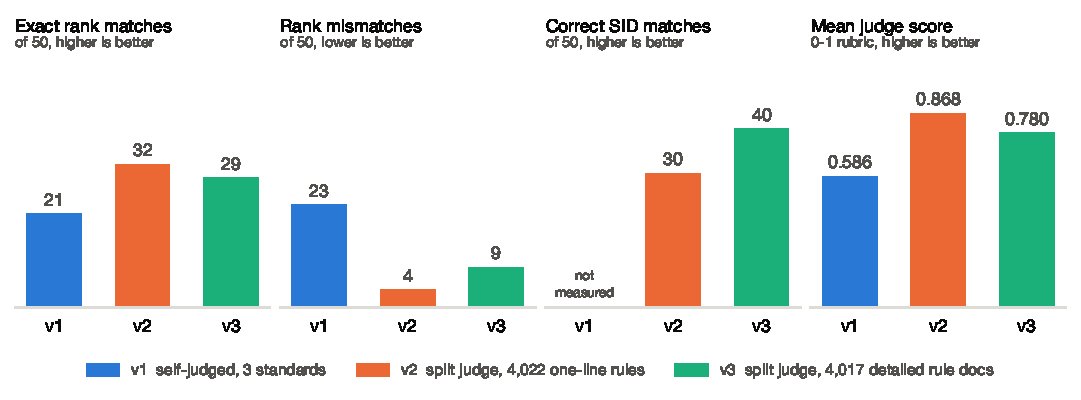
\includegraphics[width=0.94\textwidth]{figures/alert_runs.pdf}
  \end{center}
  \vspace{-0.3em}
  \lede{Exact matches 32 $\rightarrow$ 29. Mismatches 4 $\rightarrow$ 9. Judge mean 0.868 $\rightarrow$ 0.780.
  Rule matching was introduced in v2, so v1 has no value to show.}
  \keytake{Richer evidence improved one thing and degraded another. Reporting only the first would have been dishonest.}
\end{frame}

% --- 23 --------------------------------------------------------------
\begin{frame}{Why the regression is over-reach, not refinement}
  \begin{columns}[T,onlytextwidth]
    \begin{column}{0.5\textwidth}
      \begin{center}
        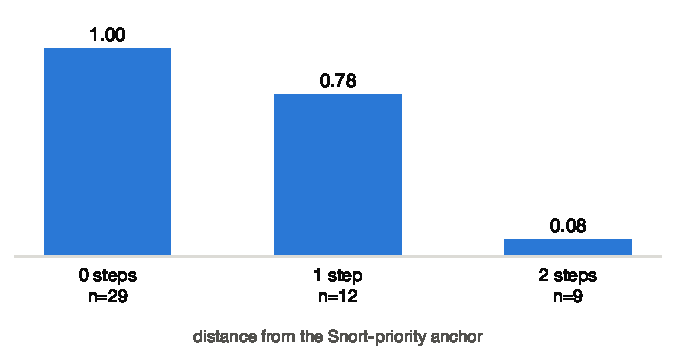
\includegraphics[width=\textwidth]{figures/judge_delta.pdf}
      \end{center}
    \end{column}
    \begin{column}{0.46\textwidth}
      {\small The rubric \emph{wants} one-step revision --- and the judge grants it: those
      12 rankings still score \textbf{0.78}.}
      \vspace{0.7em}

      {\small Two-step departures score \textbf{0.08}. Seven of the nine are a flat zero.
      The judge, which sees ground truth, rejects essentially all of them.}
      \vspace{0.7em}

      {\small \textbf{The cause:} with CVE text and rule explanations now in context, the
      ranker weighs narrative severity --- ``CVSS 10.0'', ``complete compromise'' --- above
      the Snort priority, and overshoots.}
    \end{column}
  \end{columns}
  \keytake{The ``revise when evidence warrants'' latitude was written for one line of rule code. It has not been re-tuned --- so this is a measured result, not a fitted one.}
\end{frame}

% --- 24 --------------------------------------------------------------
\begin{frame}{What this system does not do}
  \begin{itemize}
    \item The benchmark asks \textbf{answerable, single-turn} questions about \textbf{one document}.
      It does not test unanswerable questions or cross-document generalisation, and its
      scores mix retrieval and generation effects.
    \item Citations identify the retrieved \textbf{page and section}, not the sentence a claim came from.
      Refusal detection still relies on a fixed string.
    \item Follow-up rewriting is shallow, absent from Streamlit, and unmeasured.
    \item In the alert experiment: the priority-3 sample is only 3 alerts from one rule;
      the correct rule is simply \textbf{not reachable} for 10 of the 50; and ISO Annex A
      control identifiers are not parsed, so that standard is under-retrieved.
    \item The v3 prompt fix is \textbf{identified but not run}.
  \end{itemize}
\end{frame}

% --- 25 --------------------------------------------------------------
\begin{frame}{How the work was done}
  \begin{columns}[T,onlytextwidth]
    \begin{column}{0.47\textwidth}
      \textbf{\color{accent}Discipline}
      \begin{itemize}
        \item {\small \textbf{117 commits}, one completed task each, committed only after its acceptance check passed.}
        \item {\small \textbf{339 offline tests}, Ruff clean.}
        \item {\small Every run \textbf{resumable} and quota-safe --- a multi-day run survives an interrupted API window.}
      \end{itemize}
    \end{column}
    \begin{column}{0.49\textwidth}
      \textbf{\color{accent}Reproducibility}
      \begin{itemize}
        \item {\small Every request, retrieved passage and verdict is snapshotted to JSONL.}
        \item {\small Both deliverables regenerate \textbf{byte-identically} from those snapshots --- with zero new API calls.}
        \item {\small Every figure in the report is generated from committed artefacts, never transcribed.}
      \end{itemize}
    \end{column}
  \end{columns}
  \keytake{The corrections are in the record too: the metric that rewarded duplicates, the self-flattering judge, the model that returned nothing without a reasoning flag.}
\end{frame}

% --- 26 --------------------------------------------------------------
\begin{frame}{Deliverables, and the next experiment}
  \begin{columns}[T,onlytextwidth]
    \begin{column}{0.52\textwidth}
      \textbf{\color{accent}Shipped}
      {\small
      \begin{itemize}\setlength{\itemsep}{1pt}
        \item Source repository, 117 tagged commits
        \item Work record (this report) + evaluation report
        \item \code{eval/final/} --- the 250-row benchmark
        \item \code{alert\_rankings\_rag.json} --- 50 records
        \item \code{alert\_ranking\_rag\_report.md}
        \item Run snapshots for every model call
      \end{itemize}}
    \end{column}
    \begin{column}{0.44\textwidth}
      \textbf{\color{accent}Next, in priority order}
      {\small
      \begin{enumerate}\setlength{\itemsep}{1pt}
        \item Tighten the anchor latitude in the ranker prompt and re-run. Prediction: the 9 two-step mismatches shrink while the 40/50 rule matching holds.
        \item Disambiguate the 10 unreachable alerts --- query terms, top-k, or a rule-doc rerank stage.
        \item Parse ISO Annex A control identifiers so that standard stops being under-retrieved.
      \end{enumerate}}
    \end{column}
  \end{columns}
  \vspace{0.5em}
  \keytake{The most useful result of the last phase is a diagnosis, not a number.}
\end{frame}

\end{document}
